Regarding human-following robots, there has been research on this issue for a long time, outstanding Schlegel {\it et al.} \cite{visionbased} used human color and contour information to conduct tracking. In the study, the characteristic information was based on the color, edges, and texture of the clothes for tracking. For regular RGB images, Li {\it et al.} \cite{detectionbasedcolor} used image segmentation based on shape and color. The exploitation of image color spaces is also studied, including the use of HSV (Hue, Saturation, Value) and D spaces in the RGB-D space of Ren {\it et al.} \cite{realtimetarget}. Based on those two parameters, the study has determined the skeleton of the subject to be monitored. With the development of machine learning, and deep learning today. Detecting people with a camera has become a lot easier. B.X.Chen {\it et al.} \cite{refchap2-fig1} proposed a pipe for following human robot based ROS using camera and CNN to detect and tracking people (see Fig.~\ref{Chap2:Fig1}).\\ 

\begin{figure}[h]
    \centering
    % \hspace*{-8mm}
    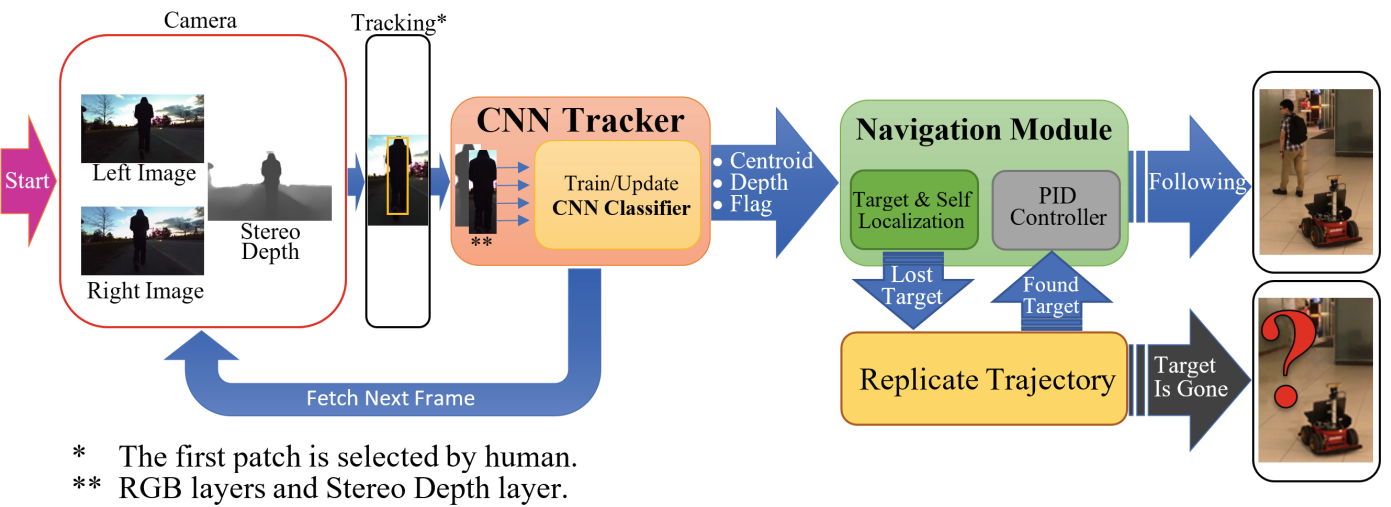
\includegraphics[width=1.0\linewidth]{figures/chap2_fig/pipeline_cnn.png}
    \caption{A Pipeline of the ROS-based Human Following Robot system using camera\cite{refchap2-fig1}}
    \label{Chap2:Fig1}
\end{figure}

In Redhwan.A and Mun-Taek.Ci's study\cite{DL_Color_feature}, the team used SSD (Single Shot Detector) to optimize human detection, combined with extracting color features in HSV space to track objects. Research using LiDAR  to determine the position of the robot as well as the position of the person in the map, as well as to identify obstacles from which it is possible to create a path from the robot position to the human position for the robot to follow.\\
% \textcolor{red}{
% You use of optimize is sometimes wrong. If you have a cost function and you use an answer that minimizes (or maximizes), you can use ``optimize''.
% In the above case, ``improve human detection accuracy'' is better.
% You did not figures in this section. You must refer the figures if you showed them. If not, you have to remove them.
% }

For the use of cameras in human-following robots, the disadvantage is that the camera has a narrow field of view, the distance for good quality is low, and it may be affected in complex environments or bad weather. Therefore, many studies have begun to use LiDAR as an alternative to the camera. Kawarazaki {\it et al.} \cite{hfr_lrs} proposed a method using LiDAR to detect human shins and obstacles around robots (see Fig.~\ref{Chap2:Fig2}). By using geometric constraints, the study was able to determine where the human shin is, thereby determining the human's position relative to the robot. The quality of the algorithm is at a good level in a simple environment. The main disadvantage of this method is that the information obtained by 2D LiDAR  is very little, so it is easy for the algorithm to confuse the human leg with other objects such as the legs of a table, chair or column. So to improve accuracy, people started using 3D LiDAR  to replace 2D LiDAR .\\

\begin{figure*}[h]
    \centering
    \begin{minipage}{\columnwidth}
        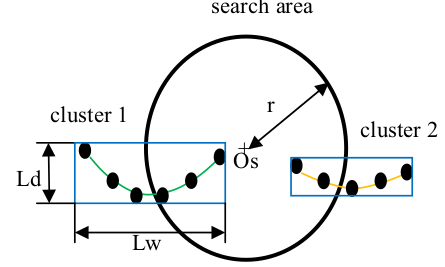
\includegraphics[width=0.48\linewidth]{figures/chap2_fig/shins_human.png}
        \hfill
        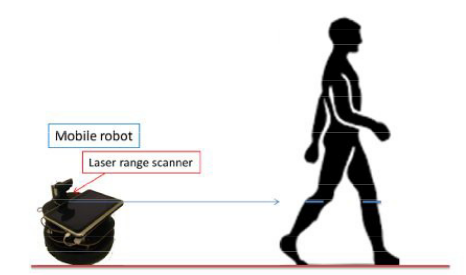
\includegraphics[width=0.48\linewidth]{figures/chap2_fig/shinshuman.png}
        \caption{Shins Human detection and following using LRS\cite{hfr_lrs}}
        \label{Chap2:Fig2}
    \end{minipage}\hfill
\end{figure*}

With 3D LiDAR , the number of point clouds that can scan objects will be much larger than with 2D LiDAR , so one can extract more features from those point clouds. One of the earliest studies on human recognition using 3D LiDAR  was by Luis {\it et al.} \cite{narvano_2009}. Research using Support Vector Machine (SVM) along with seven features. The downside of the study is that it can only detect people standing, not moving, and over short distances. Then in 2011, Kiyosumi Kidono {\it et al.} \cite{kidono}proposed two new features, the Slice feature and the Distributeion of Reflection Intensities. This proposal has somewhat solved the problem of distance and accuracy of detecting people, but there are still disadvantages such as posture or movement of people (see Fig.~\ref{Chap2:Fig3}). To solve those problems, Zhi Yan {\it et al.} \cite{online_learning}has inherited previous studies and added a tracker that helps the algorithm to detect and track moving objects. Removing some features helps to speed up computation. And especially, adding an online learning algorithm has solved the problem of accuracy in detecting people, as well as improving the algorithm when it is possible to continuously update new parameters to increase detection ability. with training time.\\

In light of the benefits and drawbacks of the earlier research approaches, we would like to provide a whole pipeline for the HFR system. The pipeline will contain model changes, user detection and tracking for online learning, input preprocessing (point-cloud), and user detection and tracking for input. We utilize PID as the control method to direct the robot to the person's designated position in the previous phase.

\begin{figure}[h]
    \centering
    % \hspace*{-8mm}
    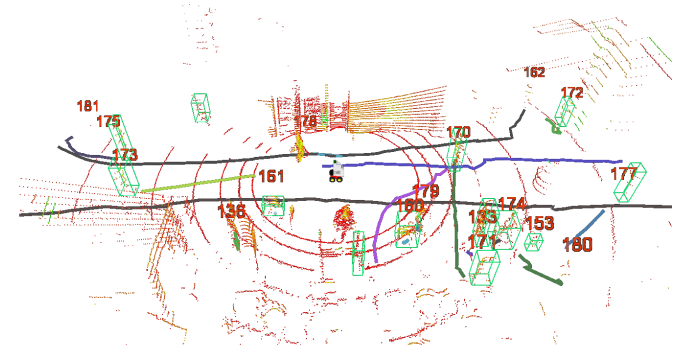
\includegraphics[scale=0.5]{figures/chap2_fig/online_learning.png}
    \caption{Human detection and tracking using Online learning with 3D LiDAR \cite{online_learning}}
    \label{Chap2:Fig3}
\end{figure}
